\documentclass{article}
\usepackage{amsmath,amssymb,amsthm,latexsym,paralist,url}
\usepackage[margin=1in]{geometry}
\usepackage{tikz}
\usetikzlibrary{arrows,automata}
\usepackage{csquotes}
\usepackage{graphicx}
\graphicspath{{images/}}
 
\theoremstyle{definition}
\newtheorem{problem}{Problem}
\newtheorem*{solution}{Solution}


\newcommand{\problemset}[1]{\begin{center}\textbf{Problem Set #1}\end{center}}


%%% HEADERS & FOOTERS
\usepackage{fancyhdr} % This should be set AFTER setting up the page geometry
\pagestyle{fancy} % options: empty , plain , fancy
\renewcommand{\headrulewidth}{0pt} % customise the layout...
\lhead{CSCE 222-501,502}
\chead{Fun Problem 5, 19 February}
\rhead{Name: Hunter Cleary}
\lfoot{}\cfoot{\thepage}\rfoot{}


\begin{document}

\noindent
Each fun problem is worth 2 Extra Credit points.\\
Due: 23 February 2018 (Friday) before 11:59pm on gradescope (\url{gradescope.com}).\\

\noindent
``But, I don't have \textit{time} for school'', explained Ada to her mother.  ``I sleep eight hours a day, which adds up to about 122 days a year.  There's no school on Saturday or Sunday, which amounts to 104 days a year.  We have 60 days of summer vacation.  I need three hours a day for meals -- thats more than 45 days a year.  And I need at least two hours of recreation every day -- that comes out to over 30 days a year.\\
\\
Ada wrote down these figures as she spoke, then she added up all the days.  They came to 361.\\
\\
\begin{tabular}{lr}
Sleep (8 hours per day) & 122\\
Saturdays and Sundays & 104\\
Summer vacation & 60\\
Meals (3 hours per day) & 45\\
Recreation (2 hours per day) & 30\\
\cline{2-2}
\multicolumn{1}{c}{Total} & 361 days
\end{tabular}\\
\\
``You see,'' continued Ada, ``that leaves me only 4 days to be sick in bed, and I haven't even taken into account the 7 school holidays that we get every year.''\\
\\
``Something's wrong here.'' mumbled Ada's mother.\\
\\
Explain what is wrong (e.g. using a Venn diagram).
\ \\
\ \\
\textbf{Venn Diagram}\ \\
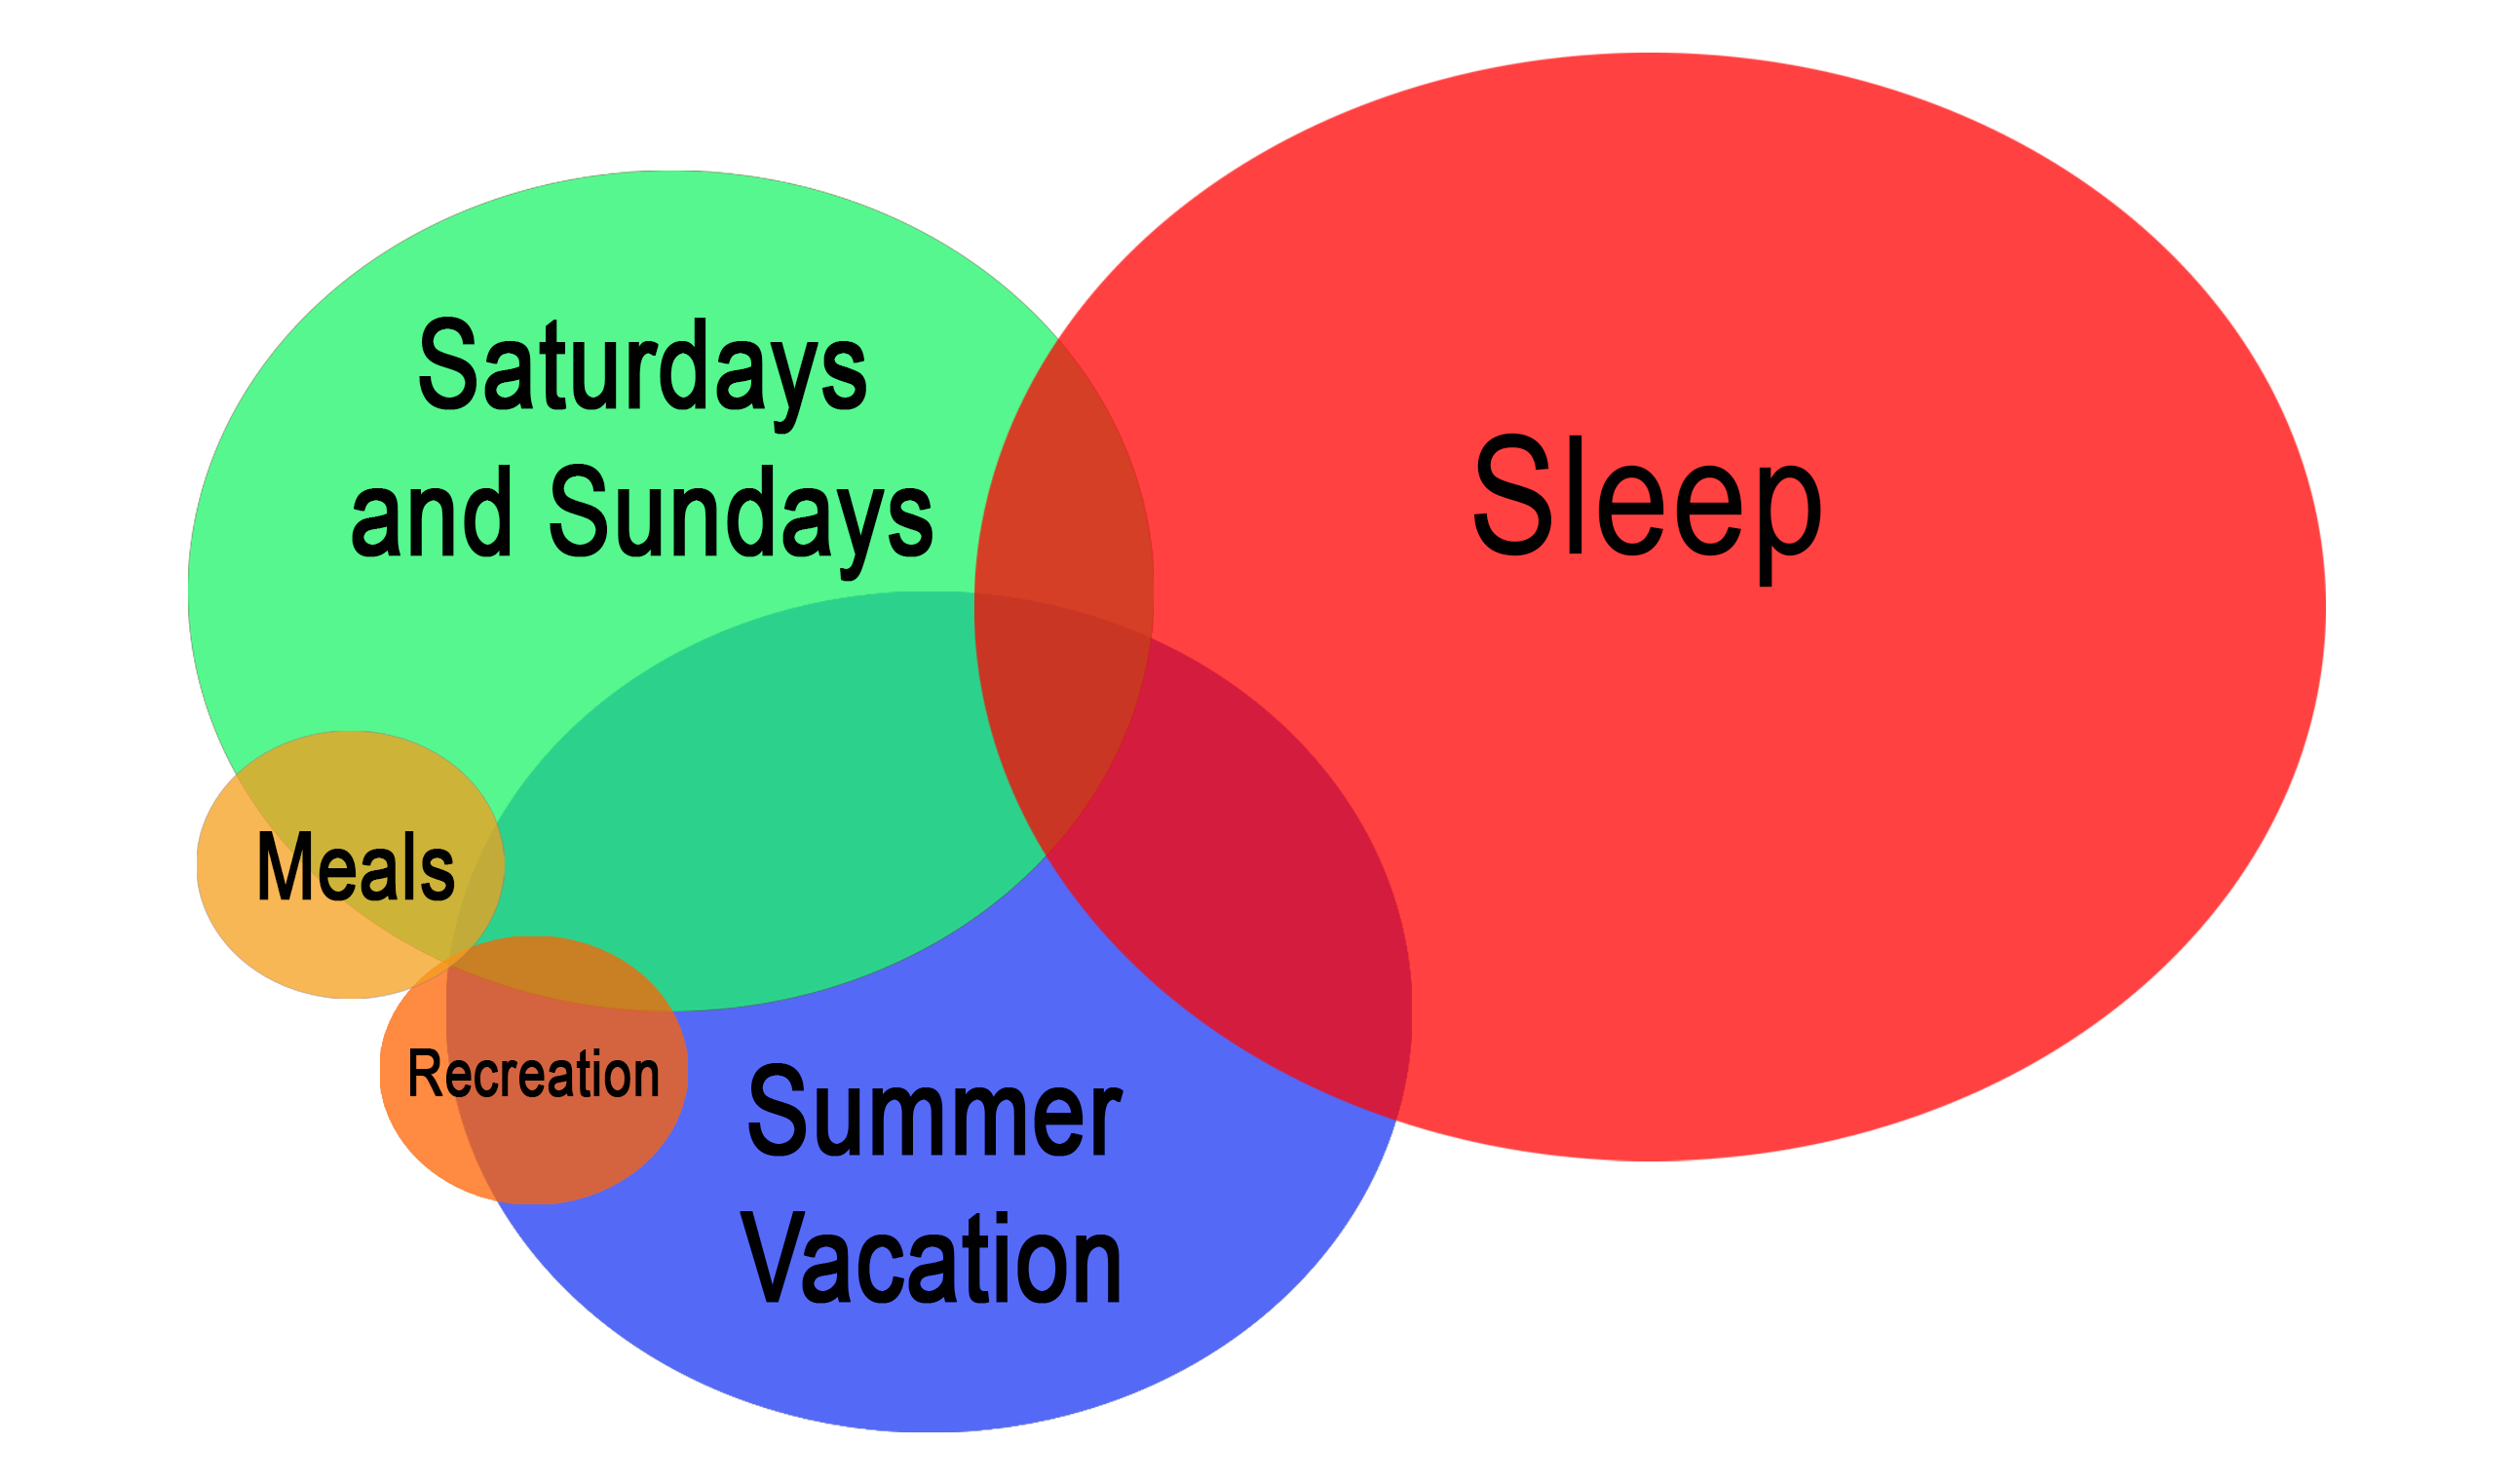
\includegraphics[width=\textwidth,height=\textheight,keepaspectratio]{VennDiagram1.png}
\ \\
Shown above is how the hours described overlap. Sleep, meals and recreation occur on every day. Summer Vacation includes a portion of the Saturdays and Sundays. Many of the times for needed activites are being accounted for multiple times and there is more than enough time for school.
\end{document}
